\section{Étape 2 : Extension du Modèle d'Assignation}

Dans cette deuxième étape, nous explorons des extensions du modèle développé dans l'étape 1. Nous cherchons à tester la capacité du modèle initial à résoudre des instances plus complexes et à explorer des configurations supplémentaires, notamment l'affectation partielle des briques et l'impact de l'augmentation de la demande, caractérisé par la création d'un nouveau poste de représentant.

\subsection{Résolution des instances 100 briques / 10 SRs}
Nous commençons par analyser la capacité du modèle initial à résoudre des instances où 100 briques doivent être assignées à 10 représentants de vente (SRs). L'objectif est de vérifier si notre modèle est capable de traiter cette augmentation de la taille du problème et de produire des solutions efficaces. On doit alors pre processer les données pour obtenir les distances entre les briques et les SRs dans le même format que l'étape 1.

\subsubsection{Modèle utilisé}
Le modèle utilisé pour cette étape est une extension du modèle multi-objectif avec epsilon-constraint présenté dans l’étape 1, avec des variables $x_{ij}$ représentant l'assignation des briques aux SRs et des distances $d_{ij}$ qui mesurent l'effort de chaque représentant en fonction des briques attribuées.

\subsubsection{Résultats obtenus}
Après résolution de l'instance avec 100 briques et 10 SRs, nous avons observé que le modèle a pu fournir une solution satisfaisante en un temps raisonnable, bien que le temps de calcul ait beaucoup augmenté par rapport à l'instance initiale de 22 zones et 4 SRs.
Et à raison : il y a 1000 variables binaires alors qu'il n'y en avait que 88 dans l'instance précédente.

\begin{figure}[H]
    \centering
    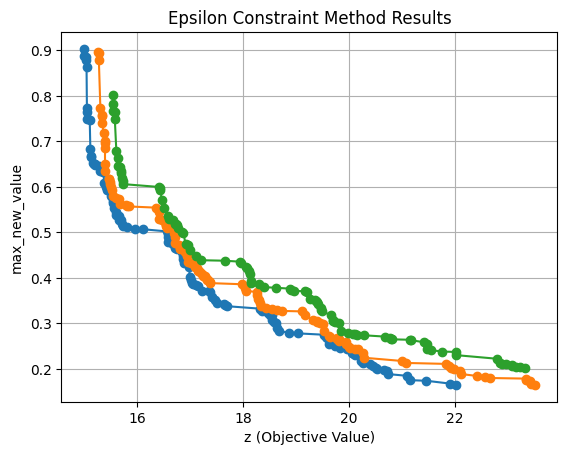
\includegraphics[width=\textwidth]{Images/step_2/step_2-min-distance.png}
    \caption{Solutions non-dominées pour 100 briques et 10 SRs}
    \label{fig:solutions_step_2}
\end{figure}

L’ensemble des solutions non-dominées (front de pareto) est représenté ci-dessus, où chaque point représente une solution obtenue pour différentes valeurs de la distance totale et de la charge de travail. On a tracé 3 courbes pour 3 niveaux de contraintes sur la charge de travail : [0.8, 1.2], [0.85, 1.15] et [0.9, 1.1].

\subsection{Modélisation de l'affectation partielle des briques}
Une autre extension que nous avons étudiée est l'affectation partielle des briques, c'est-à-dire la possibilité d'assigner une brique à plusieurs SRs. Cette modélisation peut offrir plus de flexibilité et de solutions intéressantes, surtout dans le cas où certaines zones ont des exigences de demande plus élevées.

\subsubsection{Modèle modifié}
Pour prendre en compte cette affectation partielle, nous avons seulement changé le type des valeurs $x_{ij}$ de binaire à continue entre 0 and 1 (non obligatoire, mais permet à notre modèle de converger plus vite ayant moins de valeurs à aller chercher)
L'objectif reste de minimiser la distance totale ainsi que la charge de travail maximale, mais cette fois-ci, les valeurs $x_{ij}$ ne sont pas forcément égales à 0 ou 1, et permettent de répartir les zones de manière plus flexible.

\subsubsection{Implémentation et comparaison des résultats}
L'implémentation de cette nouvelle possibilité a été réalisée de manière similaire à celle du modèle précédent, en utilisant l'optimiseur GUROBI pour résoudre le problème. La comparaison des résultats obtenus avec et sans affectation partielle montre que l'affectation partielle permet de réduire la distance totale dans certains cas, mais augmente grandement la complexité du modèle.
En effet, nous sommes passées de 1000 variables binaires (0 ou 1) à 1000 variables continues (nombre réel entre 0 et 1), ce qui augmente grandement le nombre de possibilités et donc le temps de calcul.


\begin{figure}[H]
    \centering
    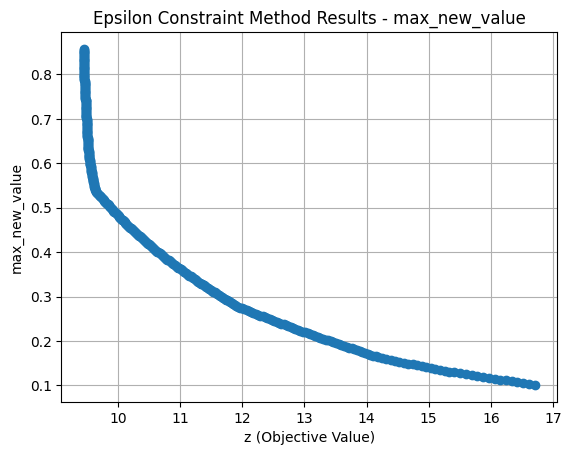
\includegraphics[width=\textwidth]{Images/step_2/step_2-new-representative-location.png}
    \caption{solutions avec affectation partielle}
    \label{fig:new_SR_location}
\end{figure}

On peut voir que le front de pareto ne comporte plus de sauts et est plus lisse, ce qui signifie que l'affectation partielle permet de trouver beaucoup plus de solutions, et est bien plus flexible.

\subsection{Impact de l'augmentation de la demande}
Supposons maintenant une augmentation uniforme de la demande dans toutes les briques, par exemple une augmentation de 25\%. Dans ce scénario, il devient nécessaire d'ajouter un nouveau représentant de vente. La question se pose alors de savoir où localiser son bureau, c'est-à-dire, quel centre de brique choisir.

Nous devons construire un modèle permettant de déterminer l'emplacement optimal du bureau du nouveau représentant, en tenant compte de la minimisation de la distance totale parcourue par l'ensemble des représentants.
Pour ce faire, nous avons modifié le modèle initial en ajoutant une nouvelle variable $y_{j}$ qui indique si le bureau du nouveau représentant est situé dans la brique $j$.
Il faudra alors rajouter et modifier des contraintes, ainsi que rajouter une colonne à $x_{ij}$ pour prendre en compte cette nouvelle variable.: 
\begin{itemize}
    \item Le bureau du nouveau représentant doit être situé dans une seule brique.
    \begin{equation}
        \sum_{j=1}^{100} y_j = 1
    \end{equation}
    \begin{equation}
        \min \sum_{i,j}^{m, n} d_{ij} x_{ij} + \sum_{jk}^{n, n} D_{kj} y_{j} x_{k, n + 1} 
    \end{equation}
    avec $D_{ij}$ la distance entre le centre de la brique $j$ et le bureau du nouveau représentant (on aura calculer chacune des possibilités en amont).

    \begin{figure}[H]
        \centering
        \begin{subfigure}[b]{0.48\textwidth}
            \centering
            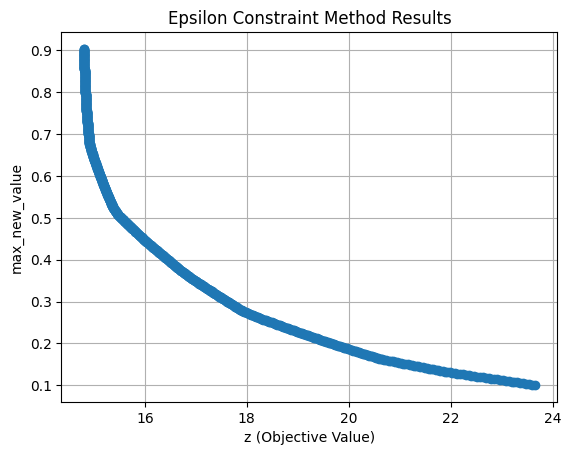
\includegraphics[width=\textwidth]{Images/step_2/step_2-pareto_front.png}
            \caption{Solutions avec affectation partielle et nouveau SR}
        \end{subfigure}
        \hfill
        \begin{subfigure}[b]{0.48\textwidth}
            \centering
            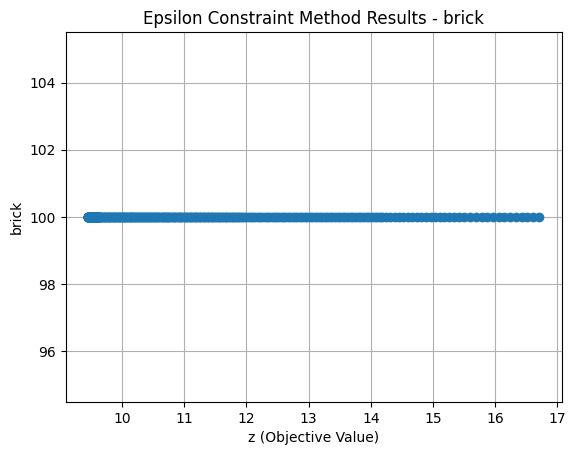
\includegraphics[width=\textwidth]{Images/step_2/step_2-pareto_front2.png}
            \caption{Numéro de la brique assigné au nouveau SR}
        \end{subfigure}
        
        \label{fig:partial_assignment_comparison}
    \end{figure}

    
\subsubsection{Résultats de l'analyse}
Après l'augmentation de la demande et l'ajout du nouveau représentant, le modèle a déterminé que le bureau du nouveau représentant devait être localisé à la 99 ieme brique, quelque soit notre emplacement sur le front de pareto.



La localisation du bureau optimal est déterminée en fonction des zones les plus sollicitées par la demande accrue, afin de minimiser la distance totale parcourue.

\subsection{Conclusion}
Dans cette étape, nous avons exploré plusieurs extensions du modèle initial, notamment la résolution d'instances plus grandes, l'affectation partielle des briques et l'impact de l'augmentation de la demande. Les résultats montrent que le modèle peut s'adapter à des problèmes de plus grande envergure, et que l'affectation partielle ainsi que l'ajout de nouveaux représentants peuvent contribuer à une meilleure répartition des charges de travail et à une minimisation de la distance totale, mais amène à une complexité de résolution grandissant énormément.

